\documentclass{beamer}
\usepackage[utf8]{inputenc}
\usepackage[T1]{fontenc}
\usepackage{amsmath}
\usepackage{graphicx}
\usepackage{xcolor}
\usepackage{hyperref}

% --- Tema y colores ---
\usetheme{Madrid}
\usecolortheme{default}

% --- Información del Documento ---
\title[Ciclos Termodinámicos]{Ciclos Termodinámicos y su Aplicación Automotriz}
\author{Profesor [Tu Nombre]}
\institute{Universidad Tecnológica de Puebla}
\date{\today}

% --- Documento ---
\begin{document}

% --- Portada ---
\begin{frame}
    \titlepage
\end{frame}

% --- Introducción a los Ciclos ---
\begin{frame}
    \frametitle{¿Qué es un Ciclo Termodinámico?}
    
    Un \alert{ciclo termodinámico} es una secuencia de procesos termodinámicos que comienzan y terminan en el mismo estado. En un ciclo, la energía neta en forma de calor ($Q$) se convierte en trabajo mecánico neto ($W$), o viceversa.
    
    \begin{itemize}
        \item \textbf{Propósito Principal:} Convertir energía térmica en trabajo útil.
        \item \textbf{Componentes Clave:}
            \begin{itemize}
                \item Procesos (isobárico, isocórico, isotérmico, adiabático).
                \item Sustancia de trabajo (ej. aire, vapor).
                \item Fuentes de calor (alta y baja temperatura).
            \end{itemize}
        \item \textbf{Relevancia Automotriz:} Son el fundamento teórico para entender el funcionamiento de los motores de combustión interna.
    \end{itemize}
\end{frame}

% --- Ciclo de Carnot ---
\begin{frame}
    \frametitle{El Ciclo Ideal: Ciclo de Carnot}
    \framesubtitle{El Límite Teórico de la Eficiencia}
    
    El ciclo de Carnot es un ciclo ideal reversible que establece la máxima eficiencia posible para cualquier motor que opere entre dos temperaturas.
    
    \textbf{Procesos del Ciclo de Carnot:}
    \begin{enumerate}
        \item Expansión isotérmica ($A \rightarrow B$)
        \item Expansión adiabática ($B \rightarrow C$)
        \item Compresión isotérmica ($C \rightarrow D$)
        \item Compresión adiabática ($D \rightarrow A$)
    \end{enumerate}
    
    \begin{columns}[T]
        \begin{column}{0.5\textwidth}
            \centering
            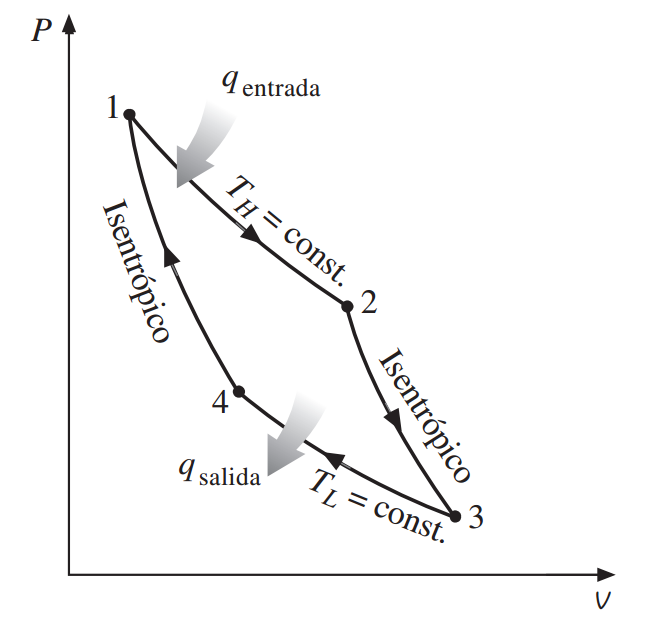
\includegraphics[width=\textwidth]{diagrama-PV-carnot.png}
            \tiny{Diagrama Presión-Volumen (P-V)}
        \end{column}
        \begin{column}{0.5\textwidth}
            \centering
            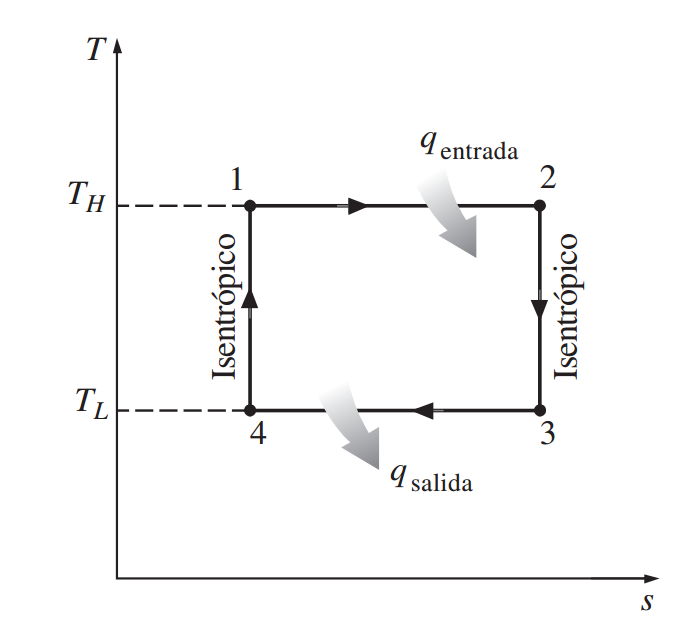
\includegraphics[width=\textwidth]{diagrama-TS-carnot.png}
            \tiny{Diagrama Temperatura-Entropía (T-S)}
        \end{column}
    \end{columns}
    
    \vspace{0.5cm}
    La eficiencia del ciclo de Carnot se define como:
    $$ \eta_{Carnot} = 1 - \frac{T_L}{T_H} $$
    Donde $T_L$ y $T_H$ son las temperaturas absolutas de los focos frío y caliente, respectivamente.
\end{frame}

% --- Ciclo Otto ---
\begin{frame}
    \frametitle{Ciclo Otto: Motores de Gasolina}
    \framesubtitle{Modelo para Motores de Encendido por Chispa (MEP)}
    
    El ciclo Otto es el modelo ideal para los motores de combustión interna de encendido por chispa.
    
    \textbf{Procesos del Ciclo Otto Ideal:}
    \begin{enumerate}
        \item Compresión adiabática ($1 \rightarrow 2$)
        \item Adición de calor a volumen constante ($2 \rightarrow 3$)
        \item Expansión adiabática (carrera de potencia) ($3 \rightarrow 4$)
        \item Rechazo de calor a volumen constante ($4 \rightarrow 1$)
    \end{enumerate}
    
    \begin{columns}[T]
        \begin{column}{0.5\textwidth}
            \centering
            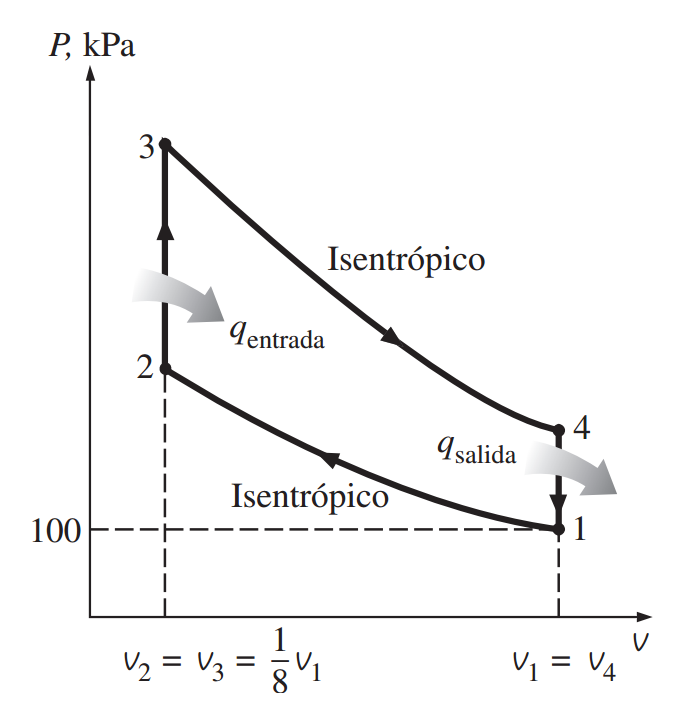
\includegraphics[width=\textwidth]{diagrama-PV-Otto.png}
            \tiny{Diagrama P-V}
        \end{column}
        \begin{column}{0.5\textwidth}
            \centering
            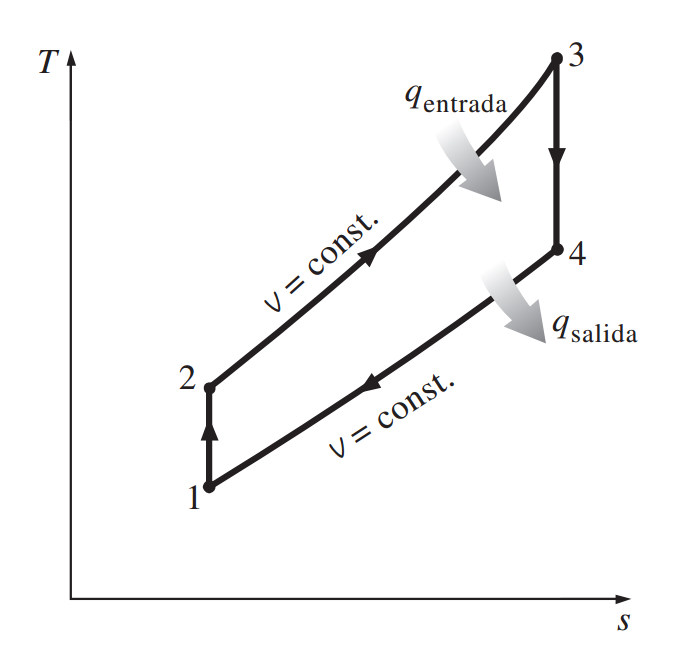
\includegraphics[width=\textwidth]{diagrama-TS-Otto.png}
            \tiny{Diagrama T-S}
        \end{column}
    \end{columns}
    
    \vspace{0.5cm}
    La eficiencia del ciclo Otto depende de la relación de compresión ($r$) y la relación de calores específicos ($k$):
    $$ \eta_{Otto} = 1 - \frac{1}{r^{k-1}} $$
    donde $r = V_1 / V_2$.
\end{frame}

% --- Ciclo Diesel ---
\begin{frame}
    \frametitle{Ciclo Diesel: Motores de Compresión}
    \framesubtitle{Modelo para Motores de Encendido por Compresión (MEC)}
    
    El ciclo Diesel modela los motores que encienden el combustible por la alta temperatura del aire comprimido.
    
    \textbf{Procesos del Ciclo Diesel Ideal:}
    \begin{enumerate}
        \item Compresión adiabática ($1 \rightarrow 2$)
        \item \alert{Adición de calor a presión constante} ($2 \rightarrow 3$)
        \item Expansión adiabática ($3 \rightarrow 4$)
        \item Rechazo de calor a volumen constante ($4 \rightarrow 1$)
    \end{enumerate}
    
    \begin{columns}[T]
        \begin{column}{0.5\textwidth}
            \centering
            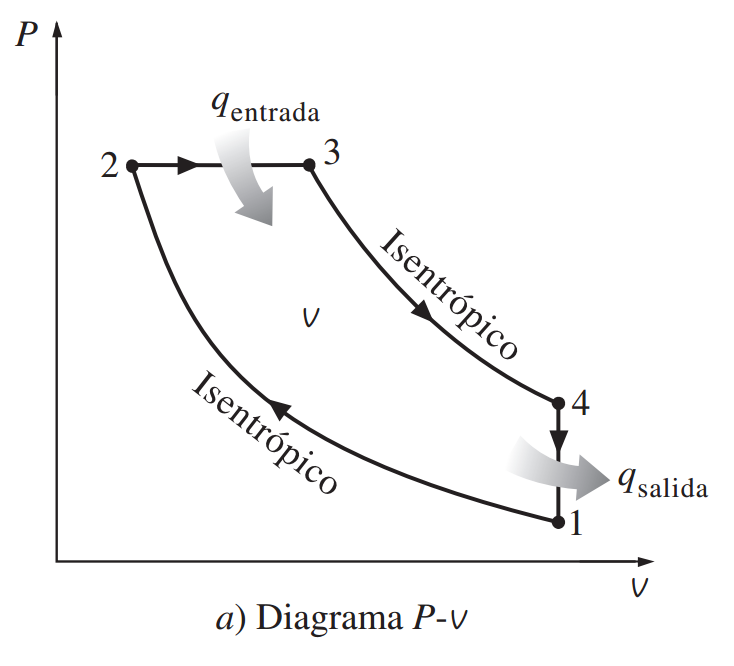
\includegraphics[width=\textwidth]{Diagrama-PV-Diesel.png}
            \tiny{Diagrama P-V}
        \end{column}
        \begin{column}{0.5\textwidth}
            \centering
            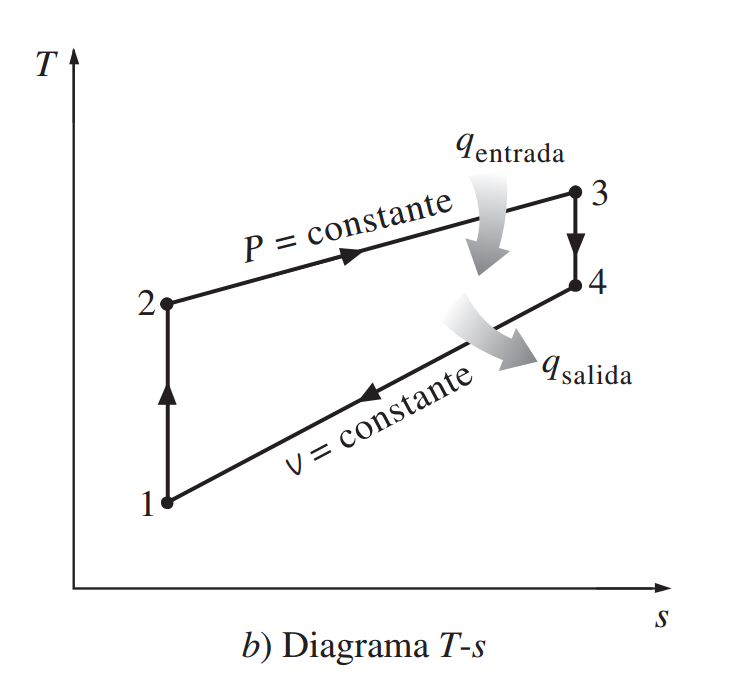
\includegraphics[width=\textwidth]{diagrama-TS-Diesel.png}
            \tiny{Diagrama T-S}
        \end{column}
    \end{columns}
    
    \vspace{0.5cm}
    La eficiencia depende de la relación de compresión ($r$) y la relación de corte ($r_c$):
    $$ \eta_{Diesel} = 1 - \frac{1}{r^{k-1}} \left[ \frac{r_c^k - 1}{k(r_c - 1)} \right] $$
    donde $r_c = V_3 / V_2$.
\end{frame}

% --- Comparación y Aplicaciones ---
\begin{frame}
    \frametitle{Comparación y Aplicaciones}
    
    \begin{block}{Puntos Clave}
        \begin{itemize}
            \item \textbf{Carnot:} Es el más eficiente teóricamente, pero \alert{no es práctico} de construir por sus procesos lentos (isotérmicos) y requerimientos de materiales. Sirve como un \textit{benchmark}.
            \item \textbf{Otto:} Menor relación de compresión para evitar la detonación (golpeteo). Característico de vehículos ligeros y de pasajeros por su alta potencia y RPM.
            \item \textbf{Diesel:} Mayor relación de compresión, lo que lleva a una mayor eficiencia. Usado en vehículos de carga, transporte pesado y maquinaria por su alto torque y economía de combustible.
        \end{itemize}
    \end{block}
    
    \begin{center}
        \textit{Para una misma relación de compresión, el ciclo Otto es más eficiente. Sin embargo, en la práctica, los motores Diesel operan a relaciones de compresión mucho mayores, resultando en una eficiencia superior.}
    \end{center}
\end{frame}

% --- Conclusiones ---
\begin{frame}
    \frametitle{Conclusiones}
    
    \begin{itemize}
        \item Los ciclos termodinámicos son herramientas esenciales para analizar y diseñar motores de combustión interna.
        \item El ciclo de \textbf{Carnot} nos da el límite superior de la eficiencia.
        \item El ciclo de \textbf{Otto} modela los motores de gasolina, donde el calor se añade a volumen constante.
        \item El ciclo de \textbf{Diesel} modela los motores diésel, donde el calor se añade a presión constante.
        \item La \alert{eficiencia} y el \alert{rendimiento} de un motor real están directamente relacionados con qué tan bien se aproxima a su ciclo ideal correspondiente.
    \end{itemize}
    
    \vspace{1cm}
    \centering
    \textbf{Siguiente paso:} Analizar las pérdidas y desviaciones de los ciclos reales respecto a los modelos ideales.
\end{frame}

% --- Preguntas ---
\begin{frame}
    \frametitle{Preguntas y Discusión}
    \begin{center}
        \Huge\bfseries
        ¿Preguntas?
    \end{center}
\end{frame}

\end{document}
